\pgfplotsset{%
  colormap={whitered}{color(0cm)=(white);
  color(1cm)=(orange!75!red)}
}
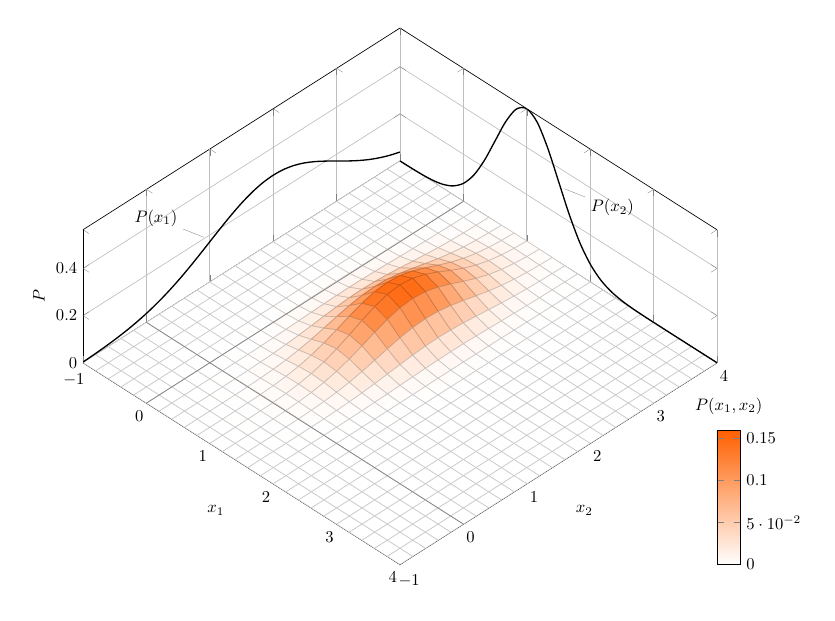
\begin{tikzpicture}[
  declare function = {mu1=1;},
  declare function = {mu2=2;},
  declare function = {sigma1=0.5;},
  declare function = {sigma2=1;},
  declare function = {normal(\m,\s)=1/(2*\s*sqrt(pi))*exp(-(x-\m)^2/(2*\s^2));},
  declare function = {bivar(\ma,\sa,\mb,\sb)=
    1/(2*pi*\sa*\sb) * exp(-((x-\ma)^2/\sa^2 + (y-\mb)^2/\sb^2))/2;},scale=0.6]
  \begin{axis}[
    colormap name  = whitered,
    width          = 15cm,
    view           = {45}{65},
    enlargelimits  = false,
    grid           = major,
    domain         = -1:4,
    y domain       = -1:4,
    samples        = 26,
    xlabel         = $x_1$,
    ylabel         = $x_2$,
    zlabel         = {$P$},
    colorbar,
    colorbar style = {
      at     = {(1,0)},
      anchor = south west,
      height = 0.25*\pgfkeysvalueof{/pgfplots/parent axis height},
      title  = {$P(x_1,x_2)$}
    }
  ]
    \addplot3 [surf] {bivar(mu1,sigma1,mu2,sigma2)};
    \addplot3 [domain=-1:4,samples=31, samples y=0, thick, smooth]
      (x,4,{normal(mu1,sigma1)});
    \addplot3 [domain=-1:4,samples=31, samples y=0, thick, smooth]
      (-1,x,{normal(mu2,sigma2)});

    \draw [black!50] (axis cs:-1,0,0) -- (axis cs:4,0,0);
    \draw [black!50] (axis cs:0,-1,0) -- (axis cs:0,4,0);

    \node at (axis cs:-1,1,0.18) [pin=165:$P(x_1)$] {};
    \node at (axis cs:1.5,4,0.32) [pin=-15:$P(x_2)$] {};
  \end{axis}
\end{tikzpicture}